\documentclass{beamer}

\usepackage[lined,ruled]{algorithm2e}
\usepackage{subfigure}
\usepackage[english]{babel}
\usepackage[latin1]{inputenc}
\usepackage{times}
\usepackage[T1]{fontenc} 
\usepackage{color}

\usetheme[secheader]{Boadilla}
\usefonttheme[onlylarge]{structurebold}
\setbeamerfont*{frametitle}{size=\normalsize,series=\bfseries}
\setbeamertemplate{navigation symbols}{}
\setbeamertemplate{mini frames}[box]
\setbeamertemplate{sections/subsections in toc}[square]
\setbeamertemplate{blocks}[rounded][shadow=true]
\setbeamertemplate{bibliography item}[text]

\setbeamercolor{lightorange}{fg=black,bg=orange!40}
\setbeamercolor{lightblue}{fg=black,bg=blue!30}

\newenvironment{colorblock}[2]
{\setbeamercolor{item}{fg=#1,bg=#1}\begin{beamerboxesrounded}[upper=#1,lower=#2,shadow=true]}
  {\end{beamerboxesrounded}}



% Setup TikZ

\usepackage{tikz}
\usetikzlibrary{arrows}
\tikzstyle{block}=[draw opacity=0.7,line width=1.4cm]


%%%%%%%%%%%%%%%%%%%%%%%%%%%%%%%%%%%%%
%%%%%%%%%%%%%%%%%%%%%%%%%%%%%%%%%%%%%
%%%%%%%%%%%%%%%%%%%%%%%%%%%%%%%%%%%%%

\newtheorem{observation}[theorem]{Observation} 

%%%%%%%%%%%%%%%%%%%%%%%%%%%%%%%%%%%%%
%%%%%%%%%%%%%%%%%%%%%%%%%%%%%%%%%%%%%
%%%%%%%%%%%%%%%%%%%%%%%%%%%%%%%%%%%%%

\title{Coordinating Distributed Systems}
\subtitle{Theory and practice}
\author{Daniele Venzano}
\institute{Eurecom}
\date


\begin{document}

\begin{frame}
  \titlepage
\end{frame}

%%%%%%%%%%%%%%%%%%%%%%%%%%%%%%%%%%%%%%%%%%%%%%%%%%%%%%%%%%
%%%%%%%%%%%%%%%%%%%%%%%%%%%%%%%%%%%%%%%%%%%%%%%%%%%%%%%%%%
\section{Introduction}

\begin{frame}
 \begin{colorblock}{blue}{lightblue}{ }
  \begin{center}
    \Huge \textbf{\texttt{Introduction}}
  \end{center}
  \end{colorblock}
\end{frame}

%%%%%%%%%%%%%%%%%%%%%%%%%%%%%%%%%%%%%%%%%%%%%%%%%%%%%%%%%%
\frame {\frametitle{Outline}
	\begin{itemize}
		\item \textbf{The consensus problem}
		\begin{itemize}
			\item A few examples of distributed consensus
			\item Eventually consistent Vs Strongly consistent, CAP theorem
			\item Fault tolerance: possible faults in distributed systems
		\end{itemize}
		
		\vspace{10pt}
		
		\item \textbf{Consensus protocols}
		\begin{itemize}
			\item Raft from A to Z
			\item Paxos overview
			\item Other protocols
		\end{itemize}
		
		\vspace{10pt}
		
		\item \textbf{Implementations - Zookeeper}
		\begin{itemize}
			\item History
			\item Architecture
			\item Data model
			\item Higher-level primitives
		\end{itemize}
			
	\end{itemize}
}
%%%%%%%%%%%%%%%%%%%%%%%%%%%%%%%%%%%%%%%%%%%%%%%%%%%%%%%%%%
%%%%%%%%%%%%%%%%%%%%%%%%%%%%%%%%%%%%%%%%%%%%%%%%%%%%%%%%%%

\section{The consensus problem}
\begin{frame}
 \begin{colorblock}{blue}{lightblue}{ }
  \begin{center}
    \Huge \textbf{\texttt{The consensus problem}}
  \end{center}
  \end{colorblock}
\end{frame}

%%%%%%%%%%%%%%%%%%%%%%%%%%%%%%%%%%%%%%%%%%%%%%%%%%%%%%%%%%
\subsection{Examples of the consensus problem}
\frame {\frametitle{Wedding consensus}
	\begin{itemize}
		\item The priest follows a well known protocol to reach a consensus:
		\begin{enumerate}
			\item Priest: Alice, will you marry Bob ?
			\item Alice: yes
			\item Priest: Bob, will you marry Alice ?
			\item Bob: yes
			\item Priest: You are now husband and wife
		\end{enumerate}

		\vspace{10pt}

		\item In distributed systems this becomes:
		\begin{enumerate}
			\item Coordinator: Alice, can you commit key X with value 5 ?
			\item Alice: yes, I can
			\item Coordinator: Bob, can you commit key X with value 5 ?
			\item Bob: yes, I can
			\item Coordinator: Ok, both of you record that X has now a value of 5
		\end{enumerate}

		\vspace{10pt}

		\item What if Bob flees from the church?
	\end{itemize}
}
%%%%%%%%%%%%%%%%%%%%%%%%%%%%%%%%%%%%%%%%%%%%%%%%%%%%%%%%%%
\frame {\frametitle{The two generals}
	\begin{center}
		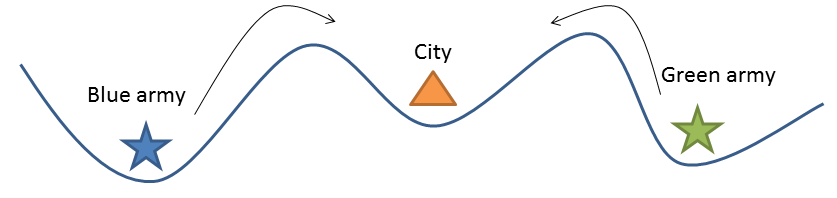
\includegraphics[width=\textwidth]{images/2generals}
	\end{center}
	\begin{itemize}
	\item Two generals want to attack a city
	\item They can only use unreliable messengers to communicate
	\item They need to attack at the same time to succeed
	\end{itemize}

	An infinite number of messages is needed for each general to be sure the other agrees on the time of the attack.
}
%%%%%%%%%%%%%%%%%%%%%%%%%%%%%%%%%%%%%%%%%%%%%%%%%%%%%%%%%%
%%%%%%%%%%%%%%%%%%%%%%%%%%%%%%%%%%%%%%%%%%%%%%%%%%%%%%%%%%

\section{Consensus protocols}

\begin{frame}
 \begin{colorblock}{blue}{lightblue}{ }
  \begin{center}
    \Huge \textbf{\texttt{Consensus protocols}}
  \end{center}
  \end{colorblock}
\end{frame}


\subsection{Paxos}
\subsection{Raft}
%%%%%%%%%%%%%%%%%%%%%%%%%%%%%%%%%%%%%%%%%%%%%%%%%%%%%%%%%%
%%%%%%%%%%%%%%%%%%%%%%%%%%%%%%%%%%%%%%%%%%%%%%%%%%%%%%%%%%

\section{Zookeper}

\begin{frame}
 \begin{colorblock}{blue}{lightblue}{ }
  \begin{center}
    \Huge \textbf{\texttt{Zookeeper}}
  \end{center}
  \end{colorblock}
\end{frame}
%%%%%%%%%%%%%%%%%%%%%%%%%%%%%%%%%%%%%%%%%%%%%%%%%%%%%%%%%%
\subsection{History}
\frame {\frametitle{History}
}
%%%%%%%%%%%%%%%%%%%%%%%%%%%%%%%%%%%%%%%%%%%%%%%%%%%%%%%%%%
\subsection{Architecture}
\frame {\frametitle{Architecture}
}
%%%%%%%%%%%%%%%%%%%%%%%%%%%%%%%%%%%%%%%%%%%%%%%%%%%%%%%%%%
\subsection{Higher-level primitives}
\frame {\frametitle{Higher-level primitives}
}

%%%%%%%%%%%%%%%%%%%%%%%%%%%%%%%%%%%%%%%%%%%%%%%%%%%%%%%%%%
%%%%%%%%%%%%%%%%%%%%%%%%%%%%%%%%%%%%%%%%%%%%%%%%%%%%%%%%%%

\section{References}
\begin{frame}[allowframebreaks]{References}
\bibliographystyle{plain} 
\end{frame}

\end{document}
